Pentru a putea executa o instructiune, aceasta trebuie citita, decodata, executa si scrise datele
inapoi in memorie. Acesti pasi au fost impartiti in componente simple, pentru a putea face
procesorul mai modular. Acesti pasi, in arhitectura clasica RISC sunt:
\begin{itemize}

\item Instruction Fetch.
\item Instruction Decode and register Fetch.
\item Execute.
\item Memory access.
\item Write Back.

\end{itemize}

\subsection{Scalar - Pipeline}

Din cauza faptului ca doar un singur modul este activ iar celelalte nu fac nimic, incepand cu ani 70
s-a folosit principul de pipeline. Astfel, pentru a se eficientiza utilizarea procesorului, mai
multe instructiuni vor fi executa in acelasi timp, dar decalate cu un pas, pentru a putea folosi
modulele mai eficient.

De exemplu, in cazul a 5 instructiuni, daca consideram ca toate stagiile dureaza 1 unitate de timp,
atunci fara pipeline ar dura 25 de unitati de timp executia totala a instructiunilor. Folosind
pipeline, timpul total de executie al celor 5 instructiuni ar fi de doar 9 unitati de timp
\cite{johnson1991superscalar}.

\begin{figure*}[ht] \centering
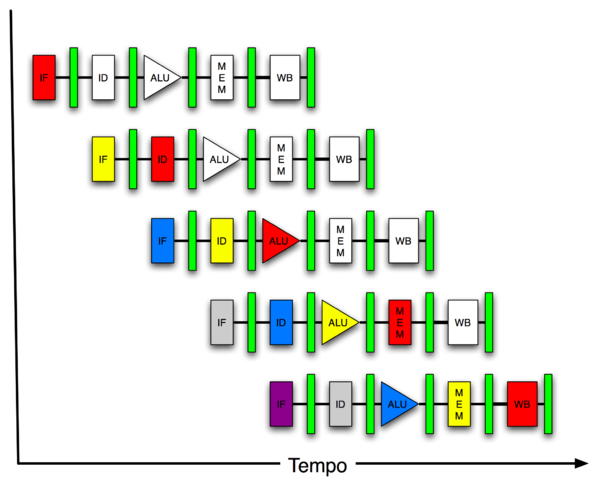
\includegraphics[width=0.9\textwidth]{img/pipeline.png}
\caption{Exemplu de executie a instructiunilor folosind pipeline.} \end{figure*}

\subsection{Scalar Avansat}

Cu timpul, odata ce unitatile interne ale procesorului au devenit din ce in ce mai puternice,
pipelineul a devenit din ce in ce mai lung, ajungand in Pentium 4 la un numar de 31 de stagii de
pipeline. Desi teoretic un pipe lung permite o granularitate mai buna, dezavantajul major il
constituie branchurile, deoarece tot pipeline-ul trebuie golit si incarcat cu instructiuni noi.
Deasemenea un pipeline mai lung inseamna o durata mai mare de executie a unei instructiuni, dar
permite atingerea unor frecvente mai mari. 

Deoarece exista unitati care pot fi nefolosite, spre exemplu floating point unit nu este
folosita cand se executa o instructiune de load sau store, dezvoltatorii de procesoare au decis sa
execute mai multe instructiuni in paralel. Astfel pipelineul pe langa numarul de stagii care le are
a fost marit si in latime. Mai exact, in loc de executia unei singuri instructiuni, se
citesc simultan mai multe instructiuni si se executa simultan. Acest mod de abordare ar permite ,
de exemplu ca in acelasi timp in care se executa adunarea a 2 registre sa se poata compara alte
registre\cite{jouppi1989available}.

\begin{figure*}[ht] \centering
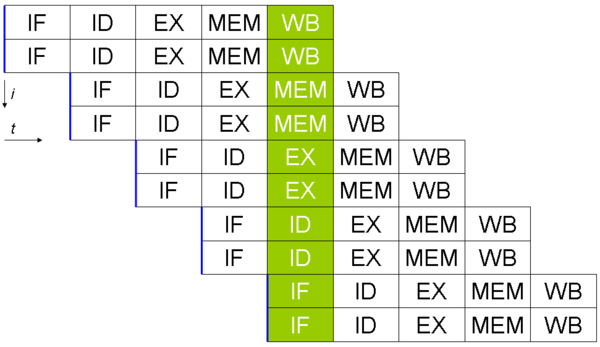
\includegraphics[width=0.9\textwidth]{img/superscalar.png}
\caption{Exemplu de executie a mai multor instructiunilor folosind super scalar.} \end{figure*}


